\chapter{State of the Art}
\label{ch:state_of_the_art}

In this chapter we will give an overview of 6D pose estimation methodologies in the state-of-the-art. Pose estimation is subject to ongoing research, as it has wide applicability in a variety of fields, including but not limited to robotics, autonomous vehicles, augmented reality and computer vision.

The methodologies supporting this issue can be divided into two main categories: learning-based and non-learning based, as explained hereafter.

\section{Non-Learning-Based Methods}
\label{s:notlearningbasedmethods}

The first pose estimation algorithms worked through image segmentation and voting schemes. In 1972, Dula and Hart started using Hough\cite{Hough} voting to detect lines and curves in images\cite{HoughLines}, and Ballard later generalised this procedure to analytically defined shapes\cite{generalisedHough}, popularizing its application for computer vision. In parallel, Lamdan and Wolfson published their Geometric Hashing\cite{GHashing} method, which is based on the representation and matching of objects using their minimal features, such as points or lines.

More modern approaches can be divided into three sub-categories. 2D-3D correspondence methods aim to recognize features in an image and match them to known object characteristics \cite{SURF}, but often rely on texture information, and cannot be applied to textureless objects. Real-image-based methods\cite{ImageMatching} transform the pose estimation problem into an image-matching problem, associating the detected image to a database of previously saved templates. This requires a difficult and time consuming process to acquire these reference images. CAD image-based methods\cite{CADMatching} aim to circumvent this by rendering the references using a 3D model. All of these approaches have issues with adapting to new situations, such as strong changes in illumination, cluttered scenes, and repeated objects.

An easy way to identify the 6D pose is through the usage of markers. When placed on an object and photographed, these markers highlight the points on the image that correspond to the 3D location of the marker, and the pose can then be obtained by solving a Perpective-n-Points\cite{PnP} (PnP) problem. For example, an ArUco marker\cite{Aruco}, can be easily and robustly detected by applying image thresholding and contour extraction, and its pose estimated by using its corners as keypoints\cite{ArucoDetection}. The obvious downside of this method is that it requires markers to be applied to objects, which is not feasible at an industrial level. Another downside is that it also does not deal with partial or total occlusions of the marker(s).

\begin{figure}[ht]
    \centering
    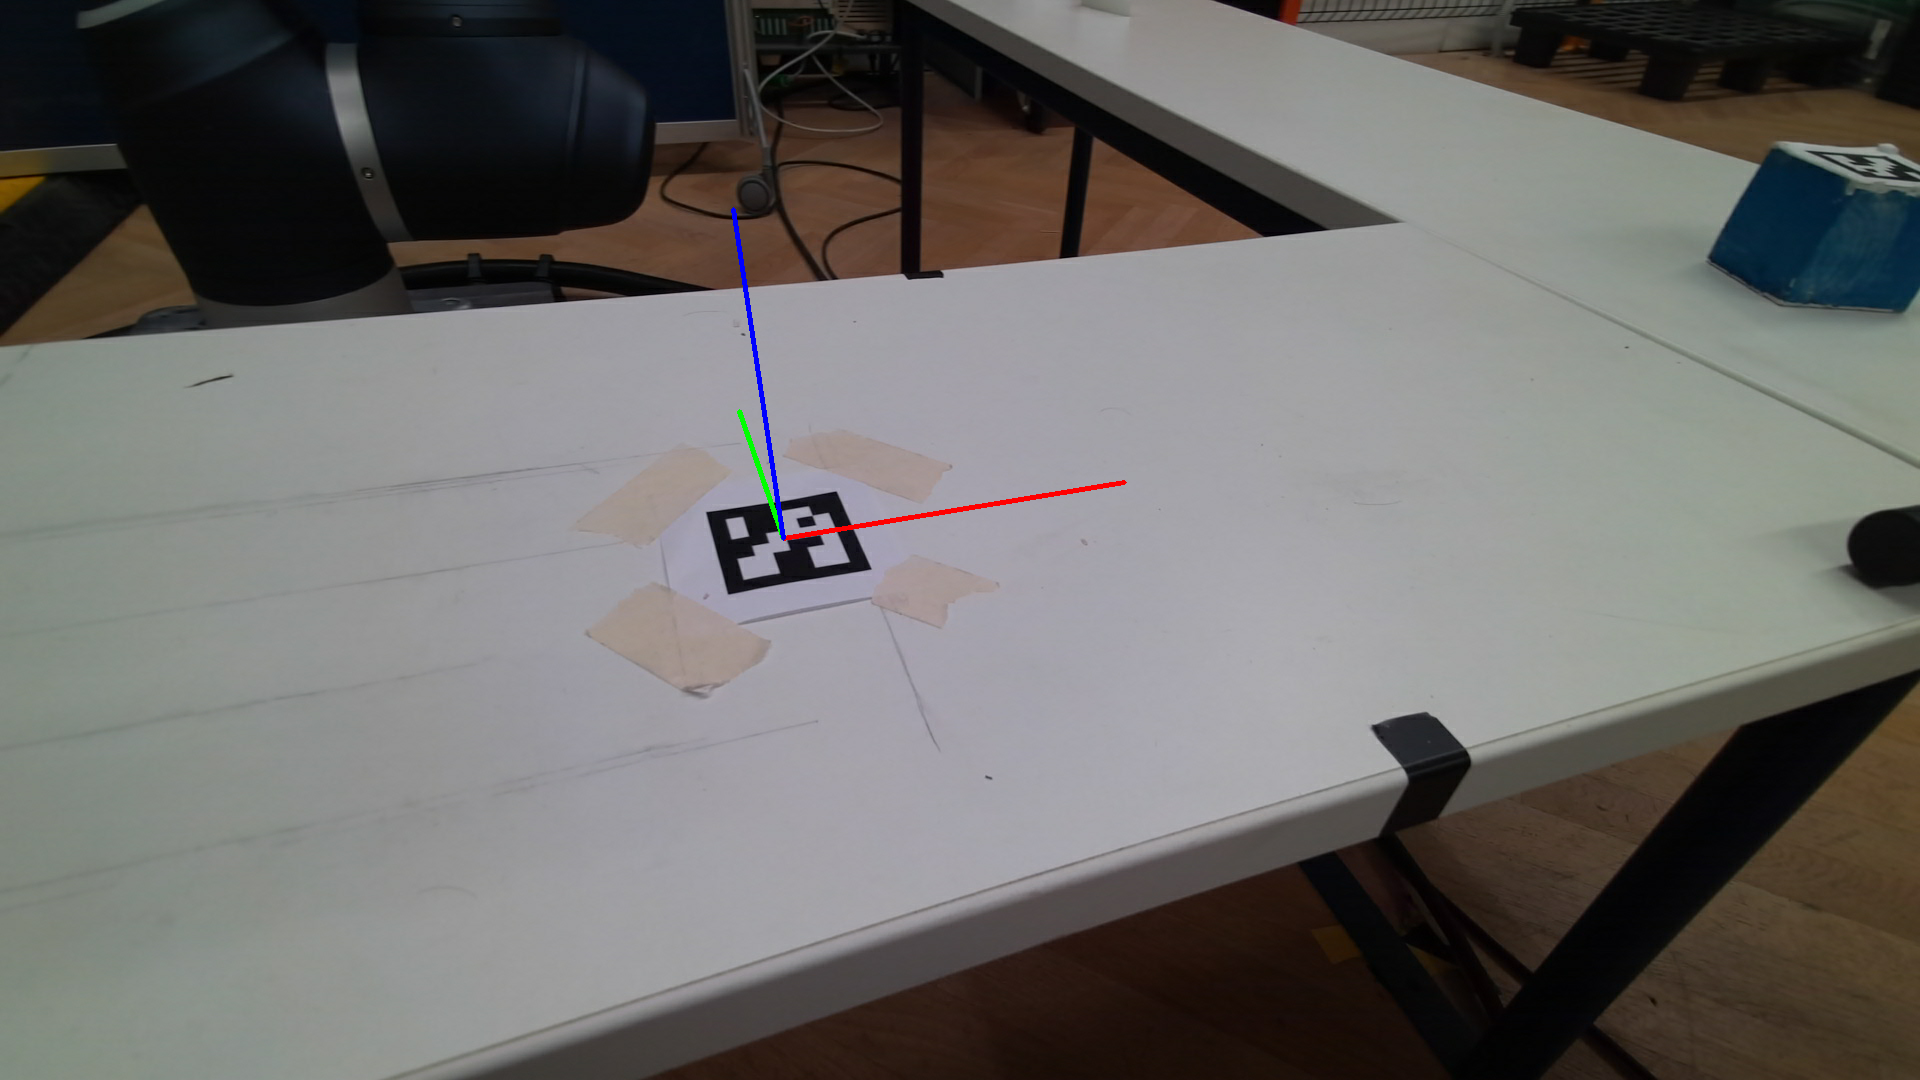
\includegraphics[width=0.6\textwidth]{output.png}
    \caption{An example of pose identification using ArUco markers.}
    \label{fig:arucoExample}
\end{figure}

Overall, non-learning based methods, while simple and computationally efficient, often require strictly controlled enviroments and specific conditions to be functional. This greatly restricts their applicability, and therefore learning-based methods are more widely used.

\section{Learning-Based Methods}
\label{s:learningbasedmethods}

Since the introduction of Convolutional Neural Networks (CNN), artifical intelligence and deep learning have been widely applied to the field of image processing, including its subfields of object detection and 6D pose estimation. The methods described in this section aim to train a CNN on vast quantities of data to perform a certain task. Based on the specifics of this task, we can categorize these approaches into three main branches: 2D-3D correspondence, direct estimation, and pose refinement. We will give a couple of examples for each of these categories.

\subsection{2D-3D Correspondence}
\label{ss:2D3D}

This class of methods uses a two step approach: they first implement a neural network to regress a set of 2-D points from an image, corresponding to a set of known feature points, and then use PnP to obtain the 6D pose of the object.

BB8\cite{BB8} uses object segmentation to perform 2D object detection, then regresses the 8 points that form the 3D bounding box of an object, but struggles with textureless symmetric or partially occluded objects. To combat these issues, PVNet\cite{PVNet} uses farthest point sampling to select keypoints on the surface of the object, and then implements a dense pixel-wise voting network, where each pixel "votes" on locations for the keypoints. RANSAC\cite{RANSAC} is then used to exclude outliers and obtain predictions with their probability distribution, which are then used for uncertainty-driven PnP.

Most approaches in this class share two common weaknesses. First, they are very perfomance-intensive when estimating the pose of multiple objects, since keypoint regression and PnP have to be computed for each object individually\cite{bukschat2020efficientpose}. Second, they are not end-to-end trainable, as the loss functions implemented do not reflect the final perfomance on the pose estimation task\cite{SS6D}. However, recent approaches have faced this issue by implementing learned or differentiable PnP algorithms, so as to enable end-to-end training\cite{EPro-Pnp}.

\subsection{Direct Estimation}
\label{ss:directestimation}

The approaches in this category exploit convolutional neural networks to directly regress the pose of an object in a single step. They are end-to-end trainable and boast better run times than the previously seen 2D-3D methods.

PoseNet\cite{PoseNet} was one of the first implementations of this concept, and was originally conceptualized for obtaining the camera pose from outdoor or indoor enviroments, and not for object pose estimation. Deep-6DPose\cite{deep6D} works by extending the Mask R-CNN\cite{Mask-R-CNN} instance segmentator, which in turn extends the Faster R-CNN\cite{Faster-R-CNN} object detector, and introduced a key technical feature by decoupling rotation and translation parameters, so as to make the pose regression loss differential. PoseCNN\cite{PoseCNN} expanded on this idea, and introduced a novel loss function that enabled it to properly handle symmetric objects.

Most networks in this category are fast and relatively accurate, but struggle in situations with partial occlusions.

\begin{table}[ht]
    \begin{center}
        \begin{tabular}{||c c c c c||} 
        \hline
        Rank & Model Name & Mean ADD & Method & Year\\ [0.5ex] 
        \hline\hline
        1 & RNNPose & 97.37 & Refinement & 2022 \\ 
        \hline
        2 & EfficientPose & 97.35 & Direct + Refinement & 2020 \\
        \hline
        3 & RePOSE & 96.1 & Refinement & 2021 \\
        \hline
        4 & EPro-PnP-6DoF v1 & 95.8 & 2D-3D & 2022\\
        \hline
        5 & ROPE & 95.61 & 2D-3D & 2021 \\
        \hline
        6 & DPOD & 95.2 & 2D-3D + Refinement & 2019\\
        \hline
        7 & HRNet  & 93.3 & 2D-3D & 2019 \\
        \hline
        8 & HybridPose & 91.3 & 2D-3D & 2020 \\
        \hline
        9 & CDPN & 89.86 & 2D-3D + Direct & 2019 \\
        \hline
        10 & PoseCNN + DeepIM & 88.6 & Direct + Refinement & 2018\\
        \hline
        \end{tabular}
    \caption{Top ten performing models on the LINEMOD dataset\cite{linemod} as of November 2022, ranked by their ADD metric (see section \ref{add_description}).}
    \label{tab:top10models}
    \end{center}
\end{table}

\subsection{Pose Refinement}
\label{ss:poserefinement}

The previously explained algorithms may only give a rough estimate of the object pose at times. If greater accuracy is required, it is often necessary to use pose refinement algorithms. Approaches in this category start from an inital estimate, and then use various methods to refine it, obtaining a more accurate prediction.

DeepIM\cite{DeepIM} employs an iterative approach, by repeatedly rendering a 3D model of the object and matching it against the observed image. To ensure successive iteraterations gain in precision, it is trained not only on an annotated dataset, but also on previous outputs of the network. RNNPose\cite{RNNPose}, while also starting from a rendering and the observed image, formulates the task as a nonlinear optimization problem: it minimizes differences between correspondence fields by leveraging recent discoveries in the field of optical flow estimation, while recurrently calling itself. RNNPose currently boasts the best performance on the widely used LINEMOD\cite{linemod} dataset by a narrow margin, as highlighted by table \ref{tab:top10models}.

While refinement methods achieve remarkable performance, they have two main downsides. First, they rely on an inital estimate of the pose, so they cannot be applied independently, and second, they are relatively computationally intensive, especially when one considers that they must be run in parallel with another estimation method to generate the initial poses.

\begin{figure}[ht]
    \centering
    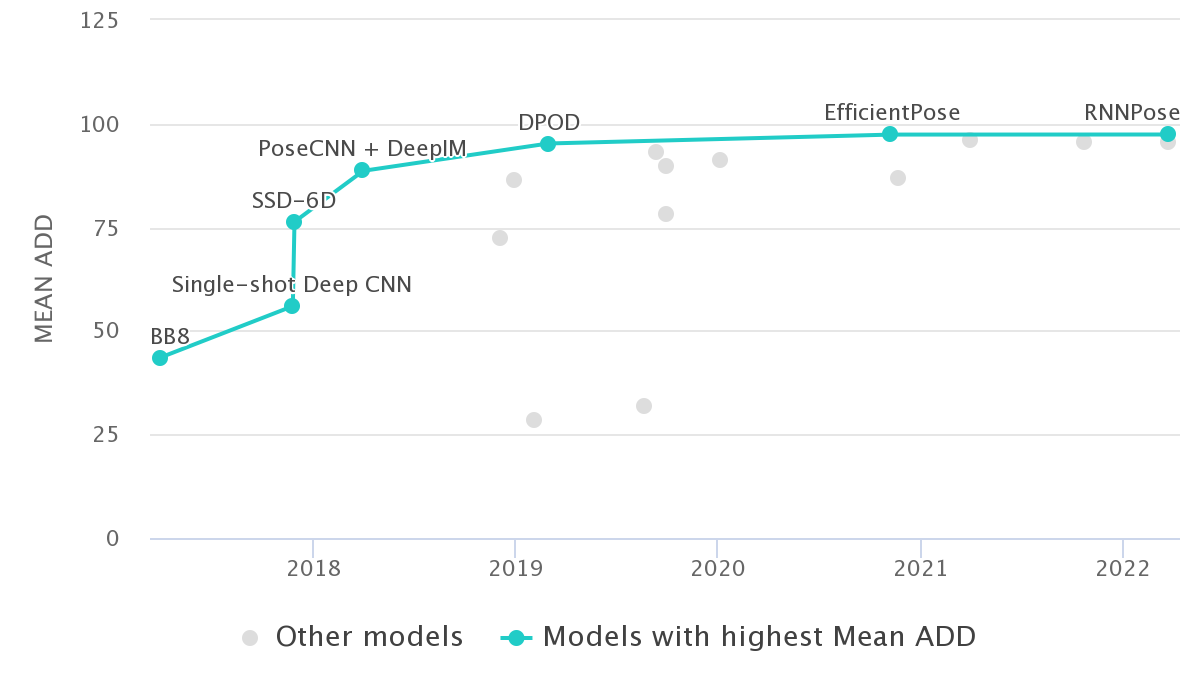
\includegraphics[width=0.7\textwidth]{linemodchart.png}
    \caption{Performance on LINEMOD of recent pose estimation algorithms by year. Graphic originates from paperswithcode.com/sota/6d-pose-estimation-on-linemod.}
    \label{fig:linemodchart}
\end{figure}

\subsection{Conclusions on Learning Approaches}

Data-driven models based on deep learning are more widely applied than non-learning-based models, as a large variety of approaches exists, and each approach brings its own distinct advantages. When choosing a model, special attention must be given to the application the model is destined for. For single object pose estimation, especially in highly occluded enviroments, 2D-3D methods are the best choice. For multi-object pose estimation, direct estimation methods provide greater computational efficency. Whenever greater accuracy is required, pose refinement algorithms offer the best results.
